\documentclass{standalone}
\usepackage{tikz}
\usetikzlibrary{patterns, positioning}
\usepackage[sfdefault]{ClearSans} %% option 'sfdefault' activates Clear Sans as the default text font
\usepackage[T1]{fontenc}

\begin{document}
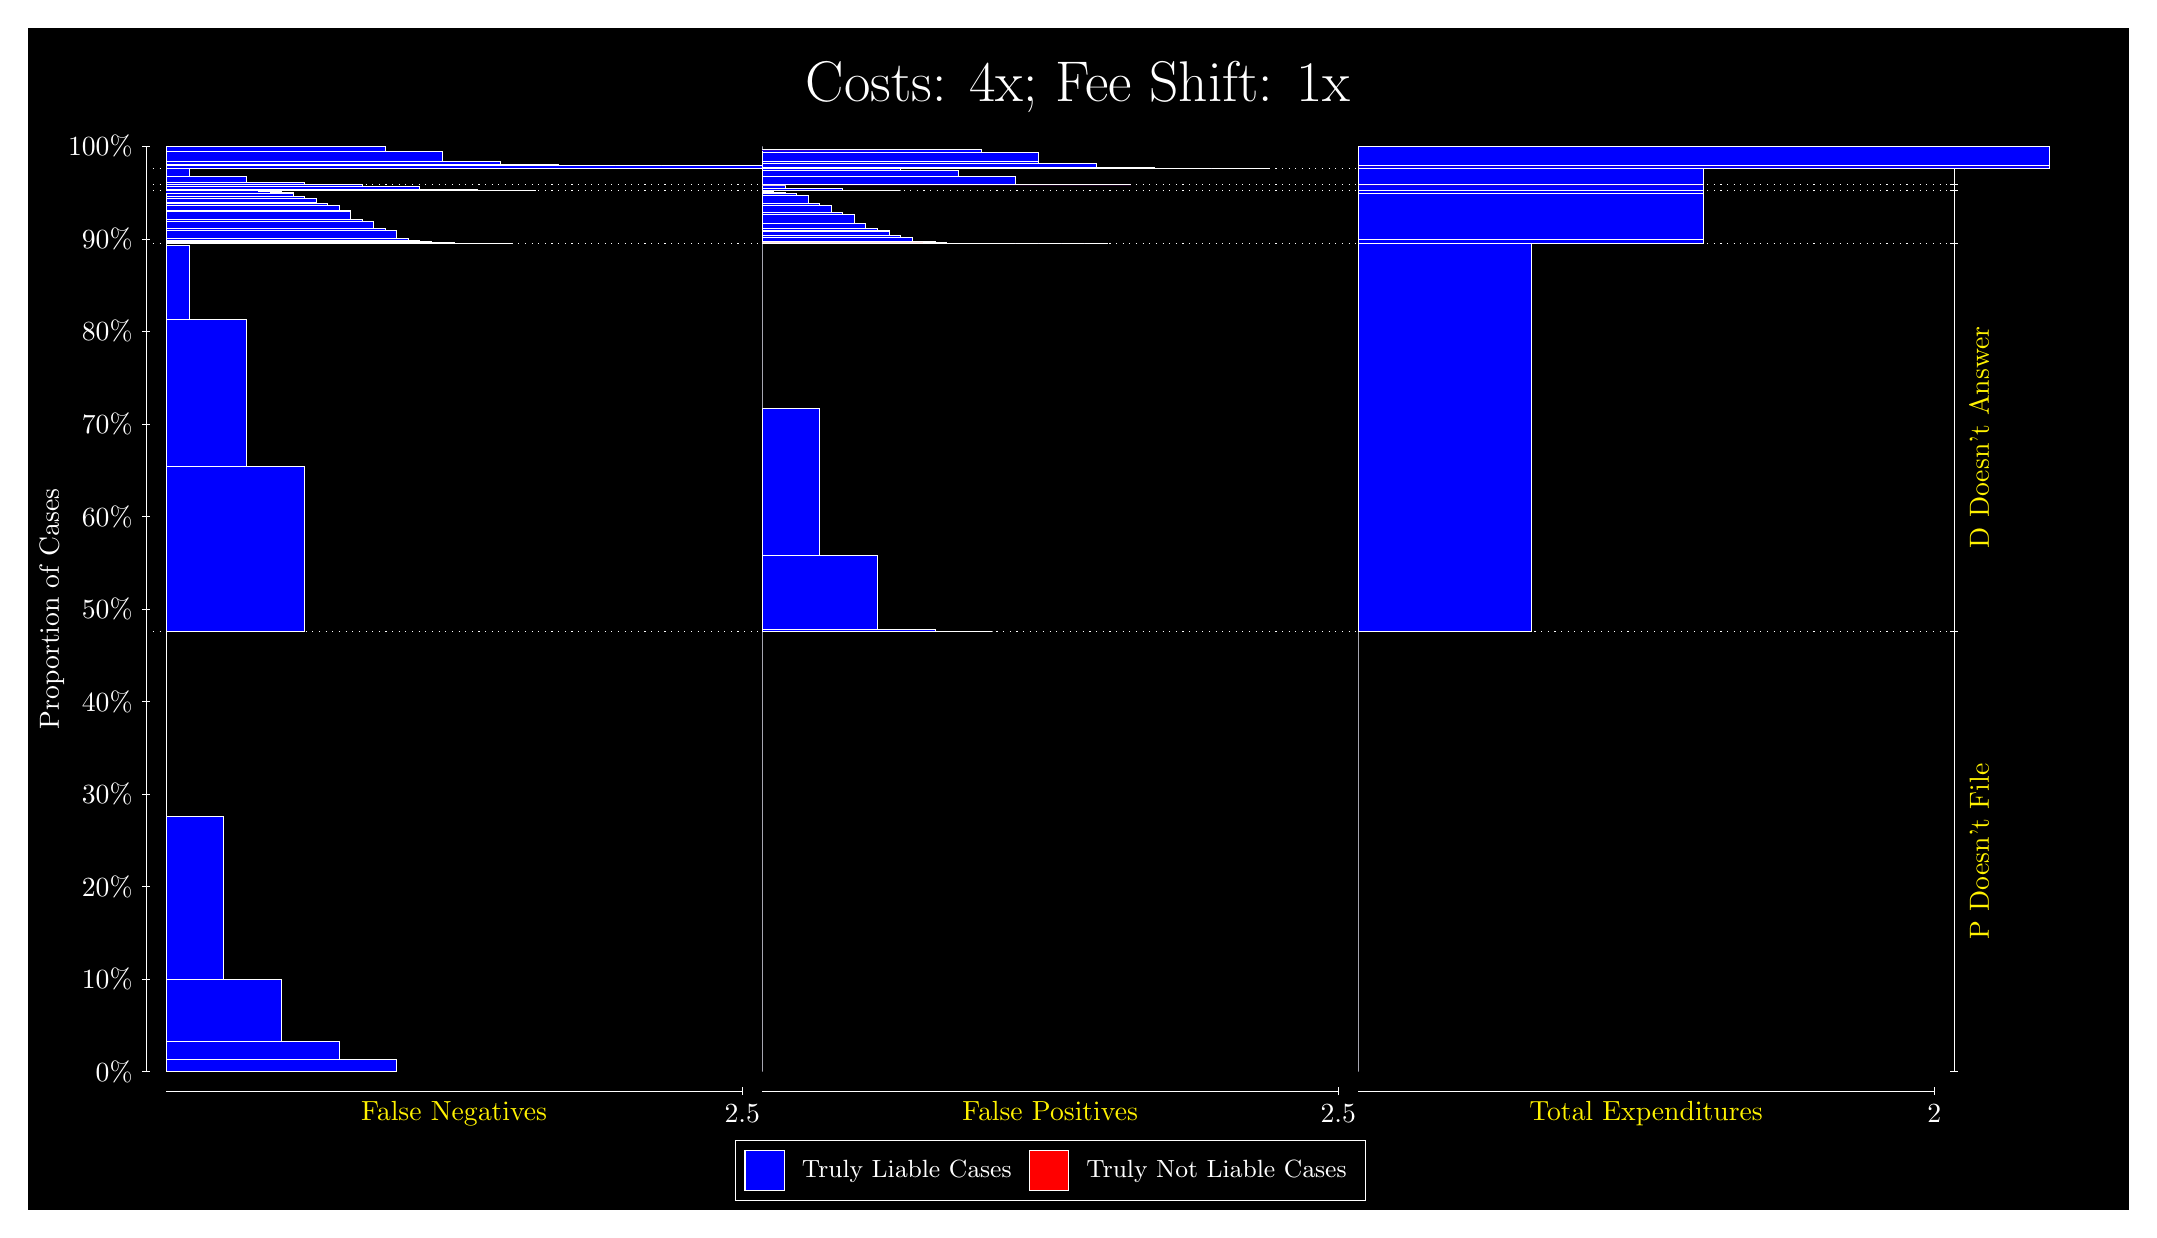
\begin{tikzpicture}
\draw[fill=black] (0,0) rectangle (26.667,15);
\draw[text=white] (0,13.5) rectangle (26.667,15) node[midway] {\huge Costs: 4x; Fee Shift: 1x};
\draw[white, very thin] (1.5,1.75) -- (1.5,13.5);
\node[rotate=90, text=white, anchor=center] at (0.3, 7.625) {Proportion of Cases};
\draw[white, very thin] (1.45,1.75) -- (1.55,1.75);
\node[text=white, anchor=east] at (1.45, 1.75) {0\%};
\draw[white, very thin] (1.45,2.925) -- (1.55,2.925);
\node[text=white, anchor=east] at (1.45, 2.925) {10\%};
\draw[white, very thin] (1.45,4.1) -- (1.55,4.1);
\node[text=white, anchor=east] at (1.45, 4.1) {20\%};
\draw[white, very thin] (1.45,5.275) -- (1.55,5.275);
\node[text=white, anchor=east] at (1.45, 5.275) {30\%};
\draw[white, very thin] (1.45,6.45) -- (1.55,6.45);
\node[text=white, anchor=east] at (1.45, 6.45) {40\%};
\draw[white, very thin] (1.45,7.625) -- (1.55,7.625);
\node[text=white, anchor=east] at (1.45, 7.625) {50\%};
\draw[white, very thin] (1.45,8.8) -- (1.55,8.8);
\node[text=white, anchor=east] at (1.45, 8.8) {60\%};
\draw[white, very thin] (1.45,9.975) -- (1.55,9.975);
\node[text=white, anchor=east] at (1.45, 9.975) {70\%};
\draw[white, very thin] (1.45,11.15) -- (1.55,11.15);
\node[text=white, anchor=east] at (1.45, 11.15) {80\%};
\draw[white, very thin] (1.45,12.325) -- (1.55,12.325);
\node[text=white, anchor=east] at (1.45, 12.325) {90\%};
\draw[white, very thin] (1.45,13.5) -- (1.55,13.5);
\node[text=white, anchor=east] at (1.45, 13.5) {100\%};

\draw[white, very thin] (24.457,1.75) -- (24.457,13.5);
\draw[white, very thin] (24.407,1.75) -- (24.507,1.75);
\node[anchor=west] at (24.407, 1.75) {};
\draw[white, very thin] (24.407,7.3416) -- (24.507,7.3416);
\node[anchor=west] at (24.407, 7.3416) {};
\draw[white, very thin] (24.407,12.267) -- (24.507,12.267);
\node[anchor=west] at (24.407, 12.267) {};
\draw[white, very thin] (24.407,12.944) -- (24.507,12.944);
\node[anchor=west] at (24.407, 12.944) {};
\draw[white, very thin] (24.407,13.015) -- (24.507,13.015);
\node[anchor=west] at (24.407, 13.015) {};
\draw[white, very thin] (24.407,13.223) -- (24.507,13.223);
\node[anchor=west] at (24.407, 13.223) {};
\draw[white, very thin] (24.407,13.5) -- (24.507,13.5);
\node[anchor=west] at (24.407, 13.5) {};

\draw[white, very thin, fill=blue] (1.75,1.75) rectangle (4.6775,1.9101);
\draw[white, very thin, fill=blue] (1.75,1.9101) rectangle (3.9457,2.1377);
\draw[white, very thin, fill=blue] (1.75,2.1377) rectangle (3.2138,2.9272);
\draw[white, very thin, fill=blue] (1.75,2.9272) rectangle (2.4819,4.9944);
\draw[white, very thin, fill=red] (1.75,4.9944) rectangle (1.75,4.9944);
\draw[white, very thin, fill=blue] (1.75,4.9944) rectangle (1.75,7.3416);
\draw[white, very thin, fill=blue] (1.75,7.3416) rectangle (3.5065,9.4415);
\draw[white, very thin, fill=blue] (1.75,9.4415) rectangle (2.7746,11.305);
\draw[white, very thin, fill=blue] (1.75,11.305) rectangle (2.0428,12.238);
\draw[white, very thin, fill=red] (1.75,12.238) rectangle (1.75,12.238);
\draw[white, very thin, fill=blue] (1.75,12.238) rectangle (1.75,12.267);
\draw[white, very thin, fill=blue] (1.75,12.267) rectangle (6.1413,12.268);
\draw[white, very thin, fill=blue] (1.75,12.268) rectangle (5.8486,12.269);
\draw[white, very thin, fill=blue] (1.75,12.269) rectangle (5.5558,12.272);
\draw[white, very thin, fill=blue] (1.75,12.272) rectangle (5.4094,12.285);
\draw[white, very thin, fill=blue] (1.75,12.285) rectangle (5.2631,12.287);
\draw[white, very thin, fill=blue] (1.75,12.287) rectangle (5.1167,12.3);
\draw[white, very thin, fill=blue] (1.75,12.3) rectangle (4.9703,12.306);
\draw[white, very thin, fill=blue] (1.75,12.306) rectangle (4.8239,12.333);
\draw[white, very thin, fill=blue] (1.75,12.333) rectangle (4.6775,12.438);
\draw[white, very thin, fill=blue] (1.75,12.438) rectangle (4.5312,12.455);
\draw[white, very thin, fill=blue] (1.75,12.455) rectangle (4.3848,12.463);
\draw[white, very thin, fill=blue] (1.75,12.463) rectangle (4.3848,12.552);
\draw[white, very thin, fill=blue] (1.75,12.552) rectangle (4.2384,12.573);
\draw[white, very thin, fill=blue] (1.75,12.573) rectangle (4.092,12.678);
\draw[white, very thin, fill=blue] (1.75,12.678) rectangle (4.092,12.683);
\draw[white, very thin, fill=blue] (1.75,12.683) rectangle (3.9457,12.752);
\draw[white, very thin, fill=blue] (1.75,12.752) rectangle (3.7993,12.782);
\draw[white, very thin, fill=blue] (1.75,12.782) rectangle (3.6529,12.794);
\draw[white, very thin, fill=blue] (1.75,12.794) rectangle (3.6529,12.839);
\draw[white, very thin, fill=blue] (1.75,12.839) rectangle (3.5065,12.861);
\draw[white, very thin, fill=blue] (1.75,12.861) rectangle (3.3602,12.905);
\draw[white, very thin, fill=blue] (1.75,12.905) rectangle (3.3602,12.912);
\draw[white, very thin, fill=blue] (1.75,12.912) rectangle (3.2138,12.923);
\draw[white, very thin, fill=blue] (1.75,12.923) rectangle (3.0674,12.924);
\draw[white, very thin, fill=blue] (1.75,12.924) rectangle (3.0674,12.931);
\draw[white, very thin, fill=blue] (1.75,12.931) rectangle (2.921,12.936);
\draw[white, very thin, fill=blue] (1.75,12.936) rectangle (2.921,12.937);
\draw[white, very thin, fill=blue] (1.75,12.937) rectangle (2.7746,12.938);
\draw[white, very thin, fill=blue] (1.75,12.938) rectangle (2.6283,12.938);
\draw[white, very thin, fill=blue] (1.75,12.938) rectangle (2.6283,12.941);
\draw[white, very thin, fill=blue] (1.75,12.941) rectangle (2.4819,12.941);
\draw[white, very thin, fill=blue] (1.75,12.941) rectangle (2.3355,12.941);
\draw[white, very thin, fill=blue] (1.75,12.941) rectangle (2.3355,12.943);
\draw[white, very thin, fill=blue] (1.75,12.943) rectangle (2.1891,12.944);
\draw[white, very thin, fill=blue] (1.75,12.944) rectangle (2.0428,12.944);
\draw[white, very thin, fill=blue] (1.75,12.944) rectangle (1.8964,12.944);
\draw[white, very thin, fill=red] (1.75,12.944) rectangle (1.75,12.944);
\draw[white, very thin, fill=blue] (1.75,12.944) rectangle (1.75,12.944);
\draw[white, very thin, fill=blue] (1.75,12.944) rectangle (6.4341,12.945);
\draw[white, very thin, fill=blue] (1.75,12.945) rectangle (5.7022,12.952);
\draw[white, very thin, fill=blue] (1.75,12.952) rectangle (4.9703,12.991);
\draw[white, very thin, fill=blue] (1.75,12.991) rectangle (4.2384,13.015);
\draw[white, very thin, fill=blue] (1.75,13.015) rectangle (3.5065,13.015);
\draw[white, very thin, fill=red] (1.75,13.015) rectangle (1.75,13.015);
\draw[white, very thin, fill=blue] (1.75,13.015) rectangle (3.5065,13.038);
\draw[white, very thin, fill=blue] (1.75,13.038) rectangle (2.7746,13.115);
\draw[white, very thin, fill=blue] (1.75,13.115) rectangle (2.0428,13.22);
\draw[white, very thin, fill=red] (1.75,13.22) rectangle (1.75,13.22);
\draw[white, very thin, fill=blue] (1.75,13.22) rectangle (1.75,13.223);
\draw[white, very thin, fill=blue] (1.75,13.223) rectangle (11.704,13.223);
\draw[white, very thin, fill=blue] (1.75,13.223) rectangle (10.972,13.223);
\draw[white, very thin, fill=blue] (1.75,13.223) rectangle (10.24,13.227);
\draw[white, very thin, fill=blue] (1.75,13.227) rectangle (9.508,13.256);
\draw[white, very thin, fill=blue] (1.75,13.256) rectangle (8.7761,13.265);
\draw[white, very thin, fill=blue] (1.75,13.265) rectangle (8.0442,13.265);
\draw[white, very thin, fill=blue] (1.75,13.265) rectangle (7.4587,13.265);
\draw[white, very thin, fill=blue] (1.75,13.265) rectangle (7.3123,13.265);
\draw[white, very thin, fill=blue] (1.75,13.265) rectangle (6.7268,13.266);
\draw[white, very thin, fill=blue] (1.75,13.266) rectangle (5.9949,13.304);
\draw[white, very thin, fill=blue] (1.75,13.304) rectangle (5.2631,13.438);
\draw[white, very thin, fill=blue] (1.75,13.438) rectangle (4.5312,13.495);
\draw[white, very thin, fill=blue] (1.75,13.495) rectangle (3.7993,13.5);
\draw[white, very thin, fill=blue] (1.75,13.5) rectangle (3.0674,13.5);
\draw[white, very thin, fill=blue] (1.75,13.5) rectangle (2.3355,13.5);
\draw[white, very thin, fill=red] (1.75,13.5) rectangle (1.75,13.5);
\draw[white, very thin, fill=red] (9.3189,1.75) rectangle (9.3189,1.75);
\draw[white, very thin, fill=blue] (9.3189,1.75) rectangle (9.3189,7.3416);
\draw[white, very thin, fill=red] (9.3189,7.3416) rectangle (12.246,7.3416);
\draw[white, very thin, fill=blue] (9.3189,7.3416) rectangle (12.246,7.3416);
\draw[white, very thin, fill=blue] (9.3189,7.3416) rectangle (11.515,7.3715);
\draw[white, very thin, fill=blue] (9.3189,7.3715) rectangle (10.783,8.3038);
\draw[white, very thin, fill=blue] (9.3189,8.3038) rectangle (10.051,10.168);
\draw[white, very thin, fill=blue] (9.3189,10.168) rectangle (9.3189,12.267);
\draw[white, very thin, fill=red] (9.3189,12.267) rectangle (13.71,12.267);
\draw[white, very thin, fill=blue] (9.3189,12.267) rectangle (13.71,12.267);
\draw[white, very thin, fill=red] (9.3189,12.267) rectangle (13.417,12.267);
\draw[white, very thin, fill=blue] (9.3189,12.267) rectangle (13.417,12.267);
\draw[white, very thin, fill=red] (9.3189,12.267) rectangle (13.125,12.267);
\draw[white, very thin, fill=blue] (9.3189,12.267) rectangle (13.125,12.267);
\draw[white, very thin, fill=blue] (9.3189,12.267) rectangle (12.978,12.268);
\draw[white, very thin, fill=red] (9.3189,12.268) rectangle (12.832,12.268);
\draw[white, very thin, fill=blue] (9.3189,12.268) rectangle (12.832,12.268);
\draw[white, very thin, fill=blue] (9.3189,12.268) rectangle (12.686,12.268);
\draw[white, very thin, fill=red] (9.3189,12.268) rectangle (12.539,12.268);
\draw[white, very thin, fill=blue] (9.3189,12.268) rectangle (12.539,12.268);
\draw[white, very thin, fill=blue] (9.3189,12.268) rectangle (12.393,12.268);
\draw[white, very thin, fill=red] (9.3189,12.268) rectangle (12.246,12.268);
\draw[white, very thin, fill=blue] (9.3189,12.268) rectangle (12.246,12.27);
\draw[white, very thin, fill=blue] (9.3189,12.27) rectangle (12.1,12.27);
\draw[white, very thin, fill=red] (9.3189,12.27) rectangle (11.954,12.27);
\draw[white, very thin, fill=blue] (9.3189,12.27) rectangle (11.954,12.274);
\draw[white, very thin, fill=blue] (9.3189,12.274) rectangle (11.807,12.274);
\draw[white, very thin, fill=red] (9.3189,12.274) rectangle (11.661,12.274);
\draw[white, very thin, fill=blue] (9.3189,12.274) rectangle (11.661,12.275);
\draw[white, very thin, fill=blue] (9.3189,12.275) rectangle (11.661,12.28);
\draw[white, very thin, fill=blue] (9.3189,12.28) rectangle (11.515,12.288);
\draw[white, very thin, fill=red] (9.3189,12.288) rectangle (11.368,12.288);
\draw[white, very thin, fill=blue] (9.3189,12.288) rectangle (11.368,12.3);
\draw[white, very thin, fill=blue] (9.3189,12.3) rectangle (11.222,12.351);
\draw[white, very thin, fill=blue] (9.3189,12.351) rectangle (11.075,12.372);
\draw[white, very thin, fill=blue] (9.3189,12.372) rectangle (10.929,12.418);
\draw[white, very thin, fill=blue] (9.3189,12.418) rectangle (10.929,12.43);
\draw[white, very thin, fill=blue] (9.3189,12.43) rectangle (10.783,12.46);
\draw[white, very thin, fill=blue] (9.3189,12.46) rectangle (10.636,12.528);
\draw[white, very thin, fill=blue] (9.3189,12.528) rectangle (10.49,12.639);
\draw[white, very thin, fill=blue] (9.3189,12.639) rectangle (10.344,12.66);
\draw[white, very thin, fill=blue] (9.3189,12.66) rectangle (10.197,12.748);
\draw[white, very thin, fill=blue] (9.3189,12.748) rectangle (10.197,12.756);
\draw[white, very thin, fill=blue] (9.3189,12.756) rectangle (10.051,12.773);
\draw[white, very thin, fill=blue] (9.3189,12.773) rectangle (9.9044,12.878);
\draw[white, very thin, fill=blue] (9.3189,12.878) rectangle (9.758,12.905);
\draw[white, very thin, fill=blue] (9.3189,12.905) rectangle (9.6116,12.911);
\draw[white, very thin, fill=blue] (9.3189,12.911) rectangle (9.4652,12.924);
\draw[white, very thin, fill=blue] (9.3189,12.924) rectangle (9.3189,12.944);
\draw[white, very thin, fill=red] (9.3189,12.944) rectangle (11.075,12.944);
\draw[white, very thin, fill=blue] (9.3189,12.944) rectangle (11.075,12.944);
\draw[white, very thin, fill=blue] (9.3189,12.944) rectangle (10.344,12.967);
\draw[white, very thin, fill=blue] (9.3189,12.967) rectangle (9.6116,13.006);
\draw[white, very thin, fill=blue] (9.3189,13.006) rectangle (9.3189,13.015);
\draw[white, very thin, fill=red] (9.3189,13.015) rectangle (14.003,13.015);
\draw[white, very thin, fill=blue] (9.3189,13.015) rectangle (14.003,13.015);
\draw[white, very thin, fill=blue] (9.3189,13.015) rectangle (13.271,13.019);
\draw[white, very thin, fill=blue] (9.3189,13.019) rectangle (12.539,13.124);
\draw[white, very thin, fill=blue] (9.3189,13.124) rectangle (11.807,13.2);
\draw[white, very thin, fill=blue] (9.3189,13.2) rectangle (11.075,13.223);
\draw[white, very thin, fill=red] (9.3189,13.223) rectangle (15.759,13.223);
\draw[white, very thin, fill=blue] (9.3189,13.223) rectangle (15.759,13.223);
\draw[white, very thin, fill=blue] (9.3189,13.223) rectangle (15.028,13.223);
\draw[white, very thin, fill=red] (9.3189,13.223) rectangle (15.028,13.223);
\draw[white, very thin, fill=blue] (9.3189,13.223) rectangle (15.028,13.223);
\draw[white, very thin, fill=blue] (9.3189,13.223) rectangle (14.296,13.226);
\draw[white, very thin, fill=red] (9.3189,13.226) rectangle (14.296,13.226);
\draw[white, very thin, fill=blue] (9.3189,13.226) rectangle (14.296,13.228);
\draw[white, very thin, fill=blue] (9.3189,13.228) rectangle (13.564,13.239);
\draw[white, very thin, fill=red] (9.3189,13.239) rectangle (13.564,13.239);
\draw[white, very thin, fill=blue] (9.3189,13.239) rectangle (13.564,13.286);
\draw[white, very thin, fill=blue] (9.3189,13.286) rectangle (12.832,13.305);
\draw[white, very thin, fill=blue] (9.3189,13.305) rectangle (12.832,13.42);
\draw[white, very thin, fill=blue] (9.3189,13.42) rectangle (12.1,13.457);
\draw[white, very thin, fill=blue] (9.3189,13.457) rectangle (11.368,13.458);
\draw[white, very thin, fill=red] (9.3189,13.458) rectangle (10.783,13.458);
\draw[white, very thin, fill=blue] (9.3189,13.458) rectangle (10.783,13.458);
\draw[white, very thin, fill=blue] (9.3189,13.458) rectangle (10.636,13.458);
\draw[white, very thin, fill=red] (9.3189,13.458) rectangle (10.051,13.458);
\draw[white, very thin, fill=blue] (9.3189,13.458) rectangle (10.051,13.458);
\draw[white, very thin, fill=red] (9.3189,13.458) rectangle (9.3189,13.458);
\draw[white, very thin, fill=blue] (9.3189,13.458) rectangle (9.3189,13.5);
\draw[white, very thin, fill=red] (16.888,1.75) rectangle (16.888,1.75);
\draw[white, very thin, fill=blue] (16.888,1.75) rectangle (16.888,7.3416);
\draw[white, very thin, fill=red] (16.888,7.3416) rectangle (19.083,7.3416);
\draw[white, very thin, fill=blue] (16.888,7.3416) rectangle (19.083,12.267);
\draw[white, very thin, fill=red] (16.888,12.267) rectangle (21.279,12.267);
\draw[white, very thin, fill=blue] (16.888,12.267) rectangle (21.279,12.317);
\draw[white, very thin, fill=red] (16.888,12.317) rectangle (21.279,12.317);
\draw[white, very thin, fill=blue] (16.888,12.317) rectangle (21.279,12.904);
\draw[white, very thin, fill=red] (16.888,12.904) rectangle (21.279,12.904);
\draw[white, very thin, fill=blue] (16.888,12.904) rectangle (21.279,12.944);
\draw[white, very thin, fill=red] (16.888,12.944) rectangle (21.279,12.944);
\draw[white, very thin, fill=blue] (16.888,12.944) rectangle (21.279,13.015);
\draw[white, very thin, fill=red] (16.888,13.015) rectangle (21.279,13.015);
\draw[white, very thin, fill=blue] (16.888,13.015) rectangle (21.279,13.223);
\draw[white, very thin, fill=red] (16.888,13.223) rectangle (25.67,13.223);
\draw[white, very thin, fill=blue] (16.888,13.223) rectangle (25.67,13.256);
\draw[white, very thin, fill=red] (16.888,13.256) rectangle (25.67,13.256);
\draw[white, very thin, fill=blue] (16.888,13.256) rectangle (25.67,13.5);
\draw[white, dotted] (1.5,7.3416) -- (24.457,7.3416);
\draw[white, dotted] (1.5,12.267) -- (24.457,12.267);
\draw[white, dotted] (1.5,12.944) -- (24.457,12.944);
\draw[white, dotted] (1.5,13.015) -- (24.457,13.015);
\draw[white, dotted] (1.5,13.223) -- (24.457,13.223);
\draw[white, very thin] (1.75,1.5) -- (9.0689,1.5);
\node[text=yellow, anchor=north] at (5.4094, 1.5) {False Negatives};
\draw[white, very thin] (9.0689,1.45) -- (9.0689,1.55);
\node[text=white, anchor=north] at (9.0689, 1.45) {2.5};

\draw[white, very thin] (9.3189,1.5) -- (16.638,1.5);
\node[text=yellow, anchor=north] at (12.978, 1.5) {False Positives};
\draw[white, very thin] (16.638,1.45) -- (16.638,1.55);
\node[text=white, anchor=north] at (16.638, 1.45) {2.5};

\draw[white, very thin] (16.888,1.5) -- (24.207,1.5);
\node[text=yellow, anchor=north] at (20.547, 1.5) {Total Expenditures};
\draw[white, very thin] (24.207,1.45) -- (24.207,1.55);
\node[text=white, anchor=north] at (24.207, 1.45) {2};

\node[text=yellow, centered, rotate=90] at (24.777, 4.5458) {P Doesn't File};
\node[text=yellow, centered, rotate=90] at (24.777, 9.8045) {D Doesn't Answer};





\draw (12.978300999999998,1.5) node[draw=none] (baseCoordinate) {};
\begin{scope}[align=center]
        \matrix[scale=0.5, draw=white, below=0.5cm of baseCoordinate, nodes={draw}, column sep=0.1cm]{
            \node[rectangle, draw, minimum width=0.5cm, minimum height=0.5cm, fill=blue] {}; &
            \node[draw=none, font=\small, text=white] (B) {Truly Liable Cases}; &
            \node[rectangle, draw, minimum width=0.5cm, minimum height=0.5cm, fill=red] {}; &
            \node[draw=none, font=\small, text=white] (B) {Truly Not Liable Cases}; \\
            };
\end{scope}

\end{tikzpicture}
\end{document}